\documentclass{article}
\usepackage[margin=0.75in]{geometry}
\usepackage[utf8]{inputenc}
\usepackage{minted}
\usepackage{caption}
\usepackage{multirow}
\usepackage{enumitem}

\title{\vspace{-1.5cm}WACC Report - Group 30}
\author{
  \begin{tabular}{ c c c c }
    Nat Karmios & Tudor-Adrian Nazarie & Austin Andrews & Joshua Jones \\
    nk4118      & tn4618        & ata2017        & jj218
  \end{tabular}
}
\date{March 2020}

\usepackage{graphicx}
\graphicspath{ {./img/} }

\begin{document}

\maketitle

% --------------------
\section{The Final Product}
% --------------------

This WACC compiler extension is a superset of the original language specification implemented in the first two milestones. As such, all automated LabTS tests from the last milestone are currently passing. Our compiler produces errors with a description of their causes and their locations in the files. The implemented extensions are discussed in section \ref{beyond}.

The compiler offers a solid basis for future development through two factors. Sealed classes allow for a finite set of classes that can be reasoned over with the \mintinline{text}{when} clause (a more-powerful variation of Java's \mintinline{text}{switch}) without having to consider an \mintinline{text}{else} branch; this allows new such classes to be added (for example, a new kind of \mintinline{text}{Type} to be introduced to the language spec) whilst making sure that it is handled every time all such types are considered. The other design choice that aids future development - just as it aided us with developing the extension - is the use of Kotlin's extension functions, to clarify the meaning of code, and clearly isolate program flow. This is particularly apparent in semantics checking and code generation, where each set of parser rules has its own \mintinline{text}{.checkSemantics()}, and each syntactic construct has a distinct \mintinline{text}{.genCode()}. This makes the behaviour of semantics checking and code generation consistent for the caller, regardless of AST node it processes on. These functions also allow us to move behaviour of a class to a different file than the class is defined in, letting us hide more niche functions from other packages where they serve no use, and organise similar groups of functions into separate files (see the \mintinline{text}{src/wacc/codegen} source directory for a good example of this).

While the compiler was written while keeping performance in mind, it is heavily affected by the reliance on the Java Virtual Machine (JVM) - when running benchmarks, optimisations to the compiler rarely had a noticeable impact, due to the time saved being negligible next to the JVM's setup time. Despite this, compilation times were still acceptable due to the simplicity of WACC as a language - see the section \ref{parallel} on parallel compilation for examples of very reasonable compilation times, even for much more substantial programs than the tests provide. One way to solve the JVM overhead issue, which was considered at the start of the project, would have been to use ANTLR to generate C sources instead of Java, include them in the Kotlin code, and compile natively. However, this was decided against, as Kotlin's native compilation is still in an experimental state.

The compiler makes three passes through the program:
\begin{enumerate}
    \item Pass through the raw file to generate lexer tokens and construct the AST (this is where ANTLR is involved).
    \item Pass through the AST to check the semantics of the user's code (and store any relevant information needed for code generation, such as the type being passed to a \mintinline{text}{print} statement.
    \item Pass through the AST to generate code, in the form of a list of objects that represent instructions.
\end{enumerate}
The number of passes is minimised to improve compilation time; fewer passes also allows for greater parallelism (see section \ref{parallel}).

% --------------------
\section{Project Management}
% --------------------

The first decision made prior to development was, of course, the language, for which Kotlin was decided; half of the group had prior experience with this language, whilst the other had none. This was a factor that had to be considered when allocating work. To alleviate this, pair programming was made use of as much as possible, which would both improve the evenness of contribution from each group member, and help the less experienced in Kotlin keep up. Aside from the ANTLR files, for which no group members had experience, this strategy was used for each stage of the project.

A downside to this structure was it created a reliance within our group that meant it was hard for some members to contribute when not all members were present. It is for that reason in-person meetups in the labs were organised as much as possible. This could have been mitigated by selecting a language more familiar to everyone - whilst Kotlin shares many similarities with Java, some of the advanced syntax it introduces made it difficult for the two group members less familiar with it to understand, though it posed an interesting additional challenge.

It was this aspect that caused issues with the development of the backend milestone; towards the deadline, there were fewer in-person lab meetups, reducing the ability of everyone to contribute, due to a lesser understanding of certain parts of the codebase. This is likely a large factor that led to not passing the tests in time.

For the extension, due to the time constraints and the additional task of getting the backend working, the group was split in two in order to complete the report on time. This also allowed us to document the different parts of our extension as they were being written.

Usage of Git was issue free; new features (at least those that would take a notable time to complete) were generally kept on separate branches during their creation to aid parallel development, though when it came to crunch time (or the occasional reformat commit), commits directly to master branch were sometimes made. For communication, a private Discord server was created. Discord is an effective means of communication as it allows for different channels to isolate separate threads of discussion. However, in-person meetings proved most beneficial to communications, so if the project were repeated, increasing the frequency of such meetings, or finding a more suitable alternative for when they were not possible, would be ideal.


% --------------------
\section{Design Choices and Implementation Details}
% --------------------

This WACC compiler was developed in Kotlin, making use of ANTLR to generate code for lexing and parsing. ANTLR was selected due to its recommendation from the course lecturers. As it generates Java source code, it was trivial to use alongside our Kotlin code, as Kotlin supports full Java interoperability. While Kotlin's native compilation was initially considered, avoiding the overhead of the JVM, involving the C source code that ANTLR can produce with Kotlin code proved too great a feat due to Kotlin/Native's experimental nature.

ANTLR aided the simplicity of lexing and parsing, as just a lexer and parser grammar file is sufficient to produce a host of useful functions and classes. Kotlin was used since its advanced syntax greatly improves readability and code organisation. For example, data classes collapse all the code necessary for a traditional Java bean into a single line.

A command line interface library, picocli \textit{(https://picocli.info/)}, was used; this is a tool that allows for development of a command line interface with minimal code. It is used it in Compile.kt, which handles the top level of the program, including command line arguments to modify the compiler's behaviour. picocli is written in Java, which, as before, makes use of Kotlin's interoperability with Java.

\begin{figure}[ht]
\centering
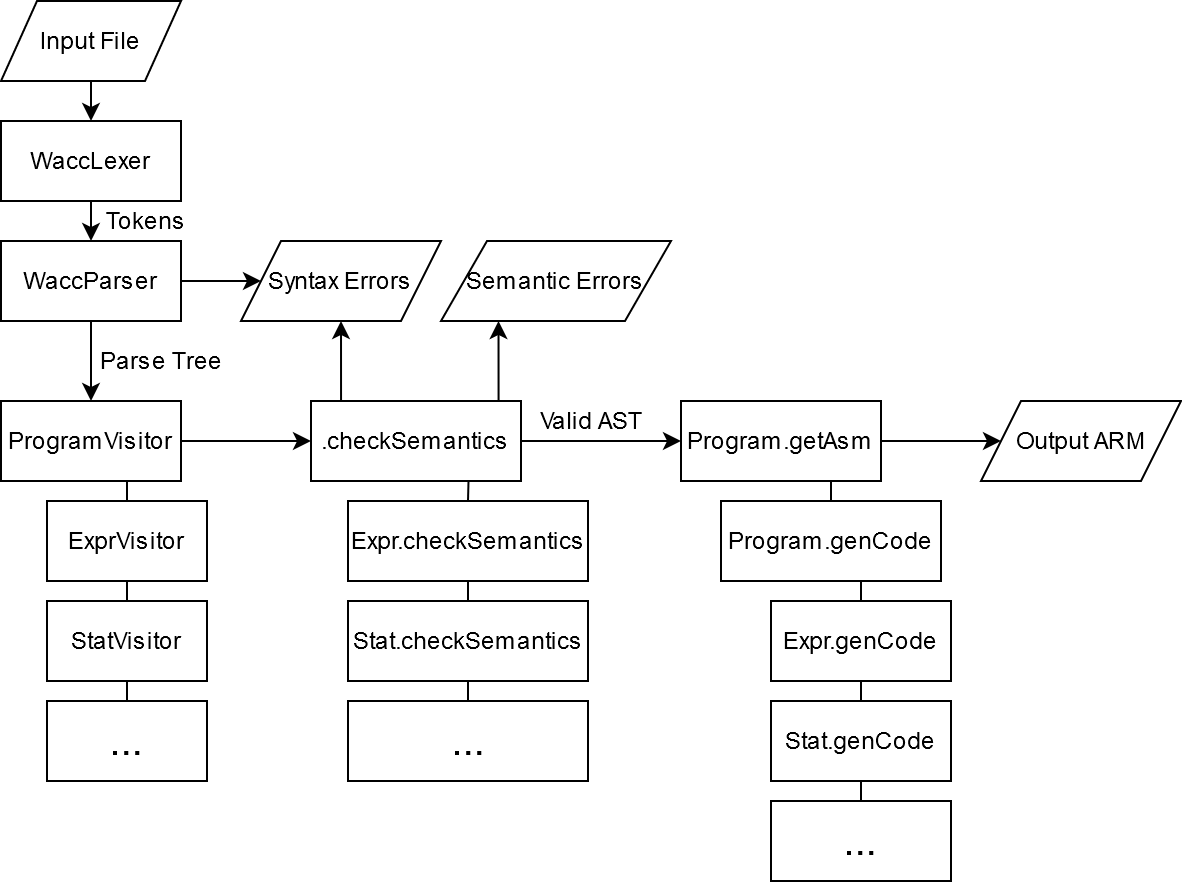
\includegraphics[scale=0.3]{compiler_structure}
\caption{The structure of the compiler}
\label{fig:compiler_structure}
\end{figure}

Development of the compiler took a primarily functional approach, rather than a more traditional object-oriented one. Because of this, it is quite difficult to align our compiler to a specific design pattern. For example, AST nodes, such as expressions, statements, etc., are all separate classes inheriting from an abstract \mintinline{text}{ASTNode} class. When assembly code is generated, for example, Kotlin's extension function syntax is used to create a case for each node type. The structure of the compiler is is described in figure \ref{fig:compiler_structure}.


% --------------------
\section{Beyond the Specification}\label{beyond}
% --------------------

\subsection{Function Overloading}

The first extension was to allow function overloading, i.e. allowing more than one function with the same name to be defined, so long as their parameters differ in some way. The core of this extension was changing how functions are identified during the compilation process; instead of just being identified by their name, they also have a \mintinline{text}{overloadIx} field, which differentiates functions of the same name. This field is assigned at the very start of the semantics check process, via the \mintinline{text}{checkOverload()} function (whilst also generating errors if a duplicate function is found).

The semantics check and code generation have thus been modified to reflect this; the semantics check, when processing an \mintinline{text}{AssignRhs.Call}, looks for a function whose parameters match the given arguments, and stores that function's \mintinline{text}{overloadIx} in the call's AST node, to be used during code generation. The code generation then use this value to select the relevant function. The function labels are also modified to differentiate them; for example, a function with name \mintinline{text}{func} and \mintinline{text}{overloadIx} 3 would have the label \mintinline{text}{f_func_3} (where it would have been \mintinline{text}{f_func} before).

An example of function overloading in WACC can be seen in \mintinline{text}{ext_examples/overload.wacc} .

\subsection{Classes}

Rudimentary classes were implemented; this mainly consisted of implementing C-style structs as well as functions that can be associated with them. Instances of a class are treated similarly to arrays, except the offset when getting or setting values is known at compile-time (thus using immediate values). For this, some new syntax structures were introduced, and others were modified:

\begin{itemize}
    \item (modified) \textbf{Program:} allow any number of Class structures to appear before function definitions
    \item (modified) \textbf{AssignRhs.Call:} allow an expression and a dot to optionally appear before the function identifier, to allow calling class methods
    \item (modified) \textbf{AssignLhs.Variable:} similarly, allow setting the values of fields in class instances
    \item (new) \textbf{Expr.ClassField:} the same, but for getting values of class instance fields
    \item (new) \textbf{Expr.Instantiate:} for creating (read: allocating memory for) a new instance of a class
    \item (new) \textbf{Type.ClassType, PairElemType.ClassType:} used to specify class types for syntax analysis; class instances should be allowed inside pairs
\end{itemize}

During semantics checking, for any of the modified AssignRhs and AssignLhs syntax, the presence of the expression and dot signifies that the identifier should be looked for in the class rather than the global function scope.

In code generation, the handling of class methods is greatly simplified by implicitly passing the relevant class instance as the first parameter, bound to \mintinline{text}{this}. Class functions are given a \mintinline{text}{cf_} prefix to their assembly labels instead of \mintinline{text}{f_} for non-class functions, to prevent any clashing.

Note that to simply handling of memory, especially when considering class instances inside arrays or pairs, all class instances are heap-allocated, and a pointer is stored in the relevant location. Because of this, \mintinline{text}{free} has been modified to allow the freeing of class instances from the heap. For completeness' sake, \mintinline{text}{print} and \mintinline{text}{println} have also been changed to support class instances, in which the memory reference is printed, similarly to how arrays and pairs are already handled.

\subsection{Code Imports}
A simple import system was implemented in the form of \mintinline{text}{include} statements. At the beginning of each WACC program, a number of \mintinline{text}{include} statements are allowed. These take the form \mintinline{text}{include <filename>.waccl;}. During compilation, each file specified in the import section of the program will be parsed and treated as a library. A library is defined as a program missing a statement to be executed; in other words, a library consists of class and function definitions and other \mintinline{text}{include} statements.

After the entire \mintinline{text}{include} dependency tree has been parsed and semantically checked, the final program is compiled. The and function definitions from the imported files are concatenated to those defined in the main program and the normal syntax checking and code generations stage takes place.

\subsection{Parallel Compilation}\label{parallel}
Since code importing had just been implemented, a natural follow-on from this was to accelerate computation via multiprocessing. At each major stage (parsing, semantics checking, code generation), there was some benefit to performance gained by multiprocessing. A divide-and-conquer approach was taken here; computation was able to be split across multiple threads in each section, like so:
\begin{itemize}
    \item \textbf{Parsing:} each file included for compilation can be parsed by ANTLR-generated code concurrently
    \item \textbf{Semantics check:} after functions have been scanned over (see overloading section), each function can be semantic-checked concurrently
    \item \textbf{Code generation:} each function can be generated concurrently
\end{itemize} 

An interesting issue was encountered when applying this method; inside the threaded task for parsing and checking a library file, the program attempts to start new tasks for semantic checking. Using a standard fixed thread pool, this works normally, however when running with 1 thread, this causes a deadlock, as the worker thread attempts to create a new thread for the sub-task, but cannot, as it is, itself, the only available thread. This was promptly solved by changing to a work-stealing pool, which is specifically designed for use cases like this.

To test this, a much larger program was compiled; this consisted of a main file and 7 included files, each consisting of 8 functions approximately 1000 lines in length each (including the main file's top-level statement). This program was compiled with a single thread, and then with the machine's full processor count (8 threads in total, in this case), 10 times each; the single-threaded compilation had an average completion time of 1434ms, whereas the multi-threaded compilation took 1286ms on average. This is a noticeable improvement, and it would only improve as the codebase grew more substantial.

\subsection{Bitwise Operators}
Several C-style bitwise operators were implemented. These were defined as binary operations, similar to addition or multiplication, with the exception of bitwise NOT, which is defined as a unary operation similar to negation. All bitwise operators operate on integers and return integers. The implemented operations are
\begin{itemize}
    \item Bitwise AND (\mintinline{text}{&})
    \item Bitwise OR (\mintinline{text}{|})
    \item Bitwise XOR (\mintinline{text}{^})
    \item Logical Shift Left (\mintinline{text}{<<})
    \item Arithmetic Shift Right (\mintinline{text}{>>})
    \item Bitwise NOT (\mintinline{text}{~})
\end{itemize}
Logical shift left was used since it is identical to arithmetic shift left. Arithmetic shift right was used in order to preserve the sign bit of the first operand.

\end{document}